\documentclass[preprint,12pt]{elsarticle}
\usepackage[T1]{fontenc}
\usepackage[utf8]{inputenc}
\usepackage{booktabs}
\usepackage{graphicx}
\usepackage{url}
\journal{Biomedical Signal Processing and Control}

\begin{document}
\begin{frontmatter}
\title{R-Peak Detection Under Electrode-Motion Noise in the MIT-BIH Noise Stress Test Database}
\author{Merve Demircio\u{g}lu}
\begin{abstract}
Electrode-motion noise can obscure R peaks and reduce the reliability of simple ECG peak detectors. This study evaluates how two fixed preprocessing approaches affect R-peak detection on the MIT-BIH Noise Stress Test Database. The 118 and 119 base recordings were examined at 0, 6, and 24 dB, yielding six signal variants rather than six independent patients. For each variant, 78 ten-second windows from the noisy intervals were evaluated at a sampling rate of 360 Hz. A raw-signal peak detector served as the baseline. The same detector was applied after a fourth-order, zero-phase 5--20 Hz Butterworth band-pass filter and after eight-level sym4 wavelet soft-thresholding. Predicted peaks were matched one-to-one with beat annotations within 150 ms. Performance was measured by pooled F1 score, with uncertainty from 1,000 paired within-record bootstrap resamples of windows. On 118e24, F1 was 0.946 for the raw baseline, 0.997 for Butterworth preprocessing, and 0.962 for wavelet preprocessing. On the 0 dB variants, Butterworth F1 was 0.620 for 118e00 and 0.576 for 119e00. The six variants share only two base recordings. As a separate fixed-parameter stress test, electrode-motion noise was synthetically added to four different MIT-BIH Arrhythmia Database base ECGs (100, 101, 103, 105). At 0 dB, pooled F1 was 0.866 for raw, 0.901 for Butterworth, and 0.876 for wavelet preprocessing; at 6 dB, corresponding values were 0.939, 0.967, and 0.953. These results provide a limited cross-record check, not clinical or population-level generalization.
\end{abstract}
\begin{keyword}
ECG \sep R-peak detection \sep electrode-motion noise \sep Butterworth filter \sep wavelet thresholding
\end{keyword}
\end{frontmatter}

\section{Introduction}
Electrode-motion artefacts can obscure ECG R peaks. This draft compares fixed preprocessing choices on the MIT-BIH Noise Stress Test Database (NSTDB) \cite{nstdb}. It is a within-record comparison, not a clinical validation.

Recent work has addressed related but distinct tasks. Rahman et al. proposed a learned noise detector that drops contaminated segments before wearable ECG classification \cite{rahman2025}. Sanz-Guerrero et al. developed an attention-based network for full-wave delineation on the 12-lead LUDB dataset \cite{sanz2026}. Costabile et al. studied a three-point weighted pre-filter before conventional ECG denoisers using signal-reconstruction metrics \cite{costabile2026}. Their datasets and endpoints differ from the NSTDB R-peak F1 comparison here; numerical scores are not directly comparable.

\section{Materials and methods}
\subsection{Data and evaluation windows}
The variants 118e00, 118e06, 118e24, 119e00, 119e06, and 119e24 derive from only two base ECG recordings. The sampling rate is 360 Hz. Each variant contributes 78 noisy ten-second windows. Beat annotations provide reference peaks.

In a separate fixed-parameter stress test, clean first-lead ECG from MIT-BIH Arrhythmia Database records 100, 101, 103, and 105 \cite{mitdb} was combined with the same 300--900 s excerpt of the NSTDB electrode-motion noise record \texttt{em} at target SNRs of 0, 6, and 24 dB. Noise was zero-meaned and scaled using the RMS of each ECG excerpt. Sixty non-overlapping ten-second windows per base record and SNR were scored. These base ECGs differ from records 118 and 119; the reused noise excerpt is not independent.

\subsection{Peak detection and preprocessing}
The raw-signal baseline uses a minimum peak distance of 0.30 s and prominence of 0.5. The identical detector is applied after a fourth-order, zero-phase 5--20 Hz Butterworth band-pass filter and after eight-level sym4 wavelet soft-thresholding. Parameters are fixed for this comparison.

\subsection{Scoring and uncertainty}
Predicted and reference peaks are matched one-to-one within $\pm150$ ms. Pooled $F_1=2TP/(2TP+FP+FN)$ is calculated by variant. Ninety-five percent confidence intervals come from 1,000 paired bootstrap resamples of windows within each original NSTDB record. The four-record stress test reports per-record and pooled descriptive F1 without confidence intervals.

\section{Results}
\begin{table}[ht]
\centering
\caption{Pooled F1 on noisy ten-second windows.}
\label{tab:f1}
\begin{tabular}{lccc}
\toprule
Variant & Raw & Butterworth & Wavelet \\
\midrule
118e00 & 0.543 & 0.620 & 0.540 \\
118e06 & 0.605 & 0.734 & 0.608 \\
118e24 & 0.946 & 0.997 & 0.962 \\
119e00 & 0.543 & 0.576 & 0.546 \\
119e06 & 0.648 & 0.706 & 0.652 \\
119e24 & 0.839 & 0.946 & 0.857 \\
\bottomrule
\end{tabular}
\end{table}
Butterworth has the highest pooled F1 point estimate in each variant (Table~\ref{tab:f1}). On 118e24, its paired difference from raw is 0.051 (95\% CI: 0.041--0.061). Wavelet thresholding does not improve on raw in every variant.

\begin{figure}[ht]
\centering
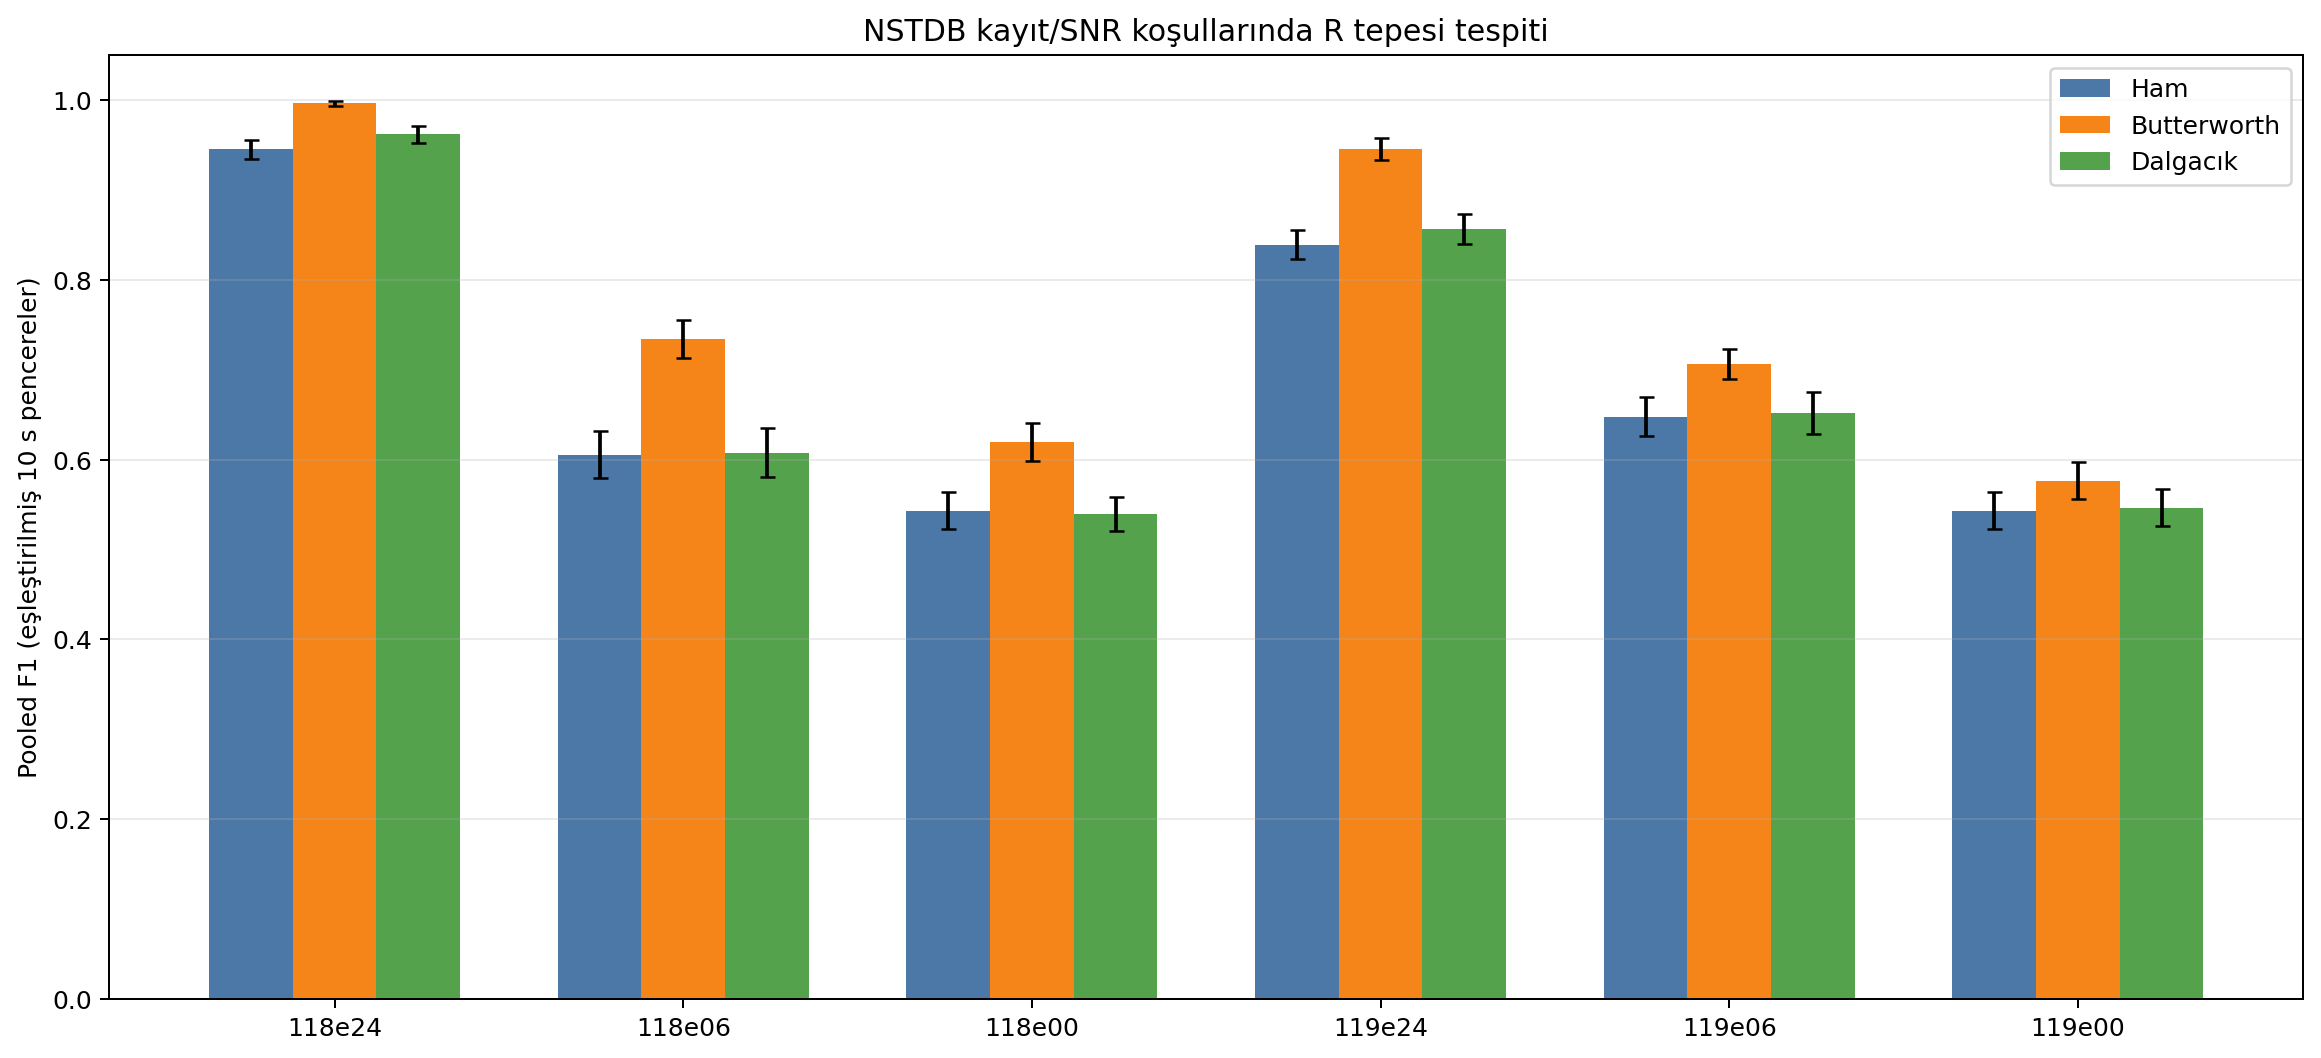
\includegraphics[width=\linewidth]{nstdb_3_yontem_f1_ga95.png}
\caption{Pooled F1 and within-record, paired-window 95\% bootstrap intervals for the three tested approaches across six NSTDB noise variants. The variants originate from two base recordings.}
\label{fig:f1}
\end{figure}
Figure~\ref{fig:f1} displays the six-variant comparison; its intervals do not represent uncertainty across independent patients.

\begin{table}[ht]
\centering
\caption{Pooled F1 across four different MIT-BIH base ECGs with synthetically added electrode-motion noise; 240 windows per SNR.}
\label{tab:external}
\begin{tabular}{lccc}
\toprule
Target SNR & Raw & Butterworth & Wavelet \\
\midrule
0 dB & 0.866 & 0.901 & 0.876 \\
6 dB & 0.939 & 0.967 & 0.953 \\
24 dB & 0.997 & 0.999 & 0.998 \\
\bottomrule
\end{tabular}
\end{table}
Butterworth had the highest pooled point estimate at each target SNR in this additional test (Table~\ref{tab:external}). It was not highest for every individual record: wavelet preprocessing scored 0.938 versus Butterworth's 0.929 on record 103 at 6 dB.

\begin{figure}[ht]
\centering
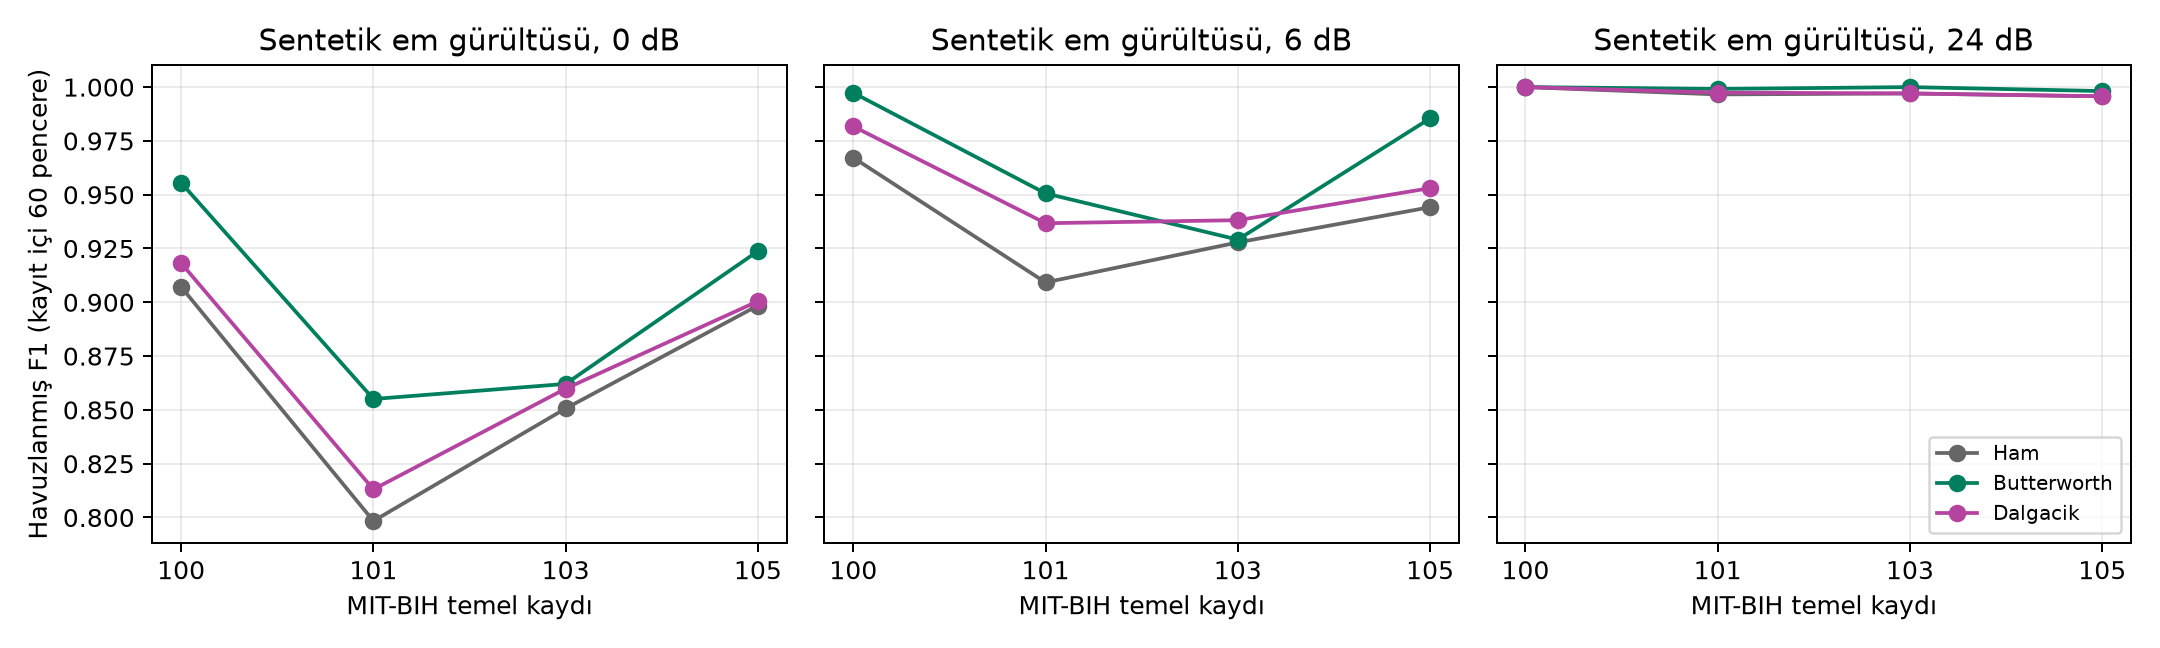
\includegraphics[width=\linewidth]{dis_dogrulama_f1.png}
\caption{Per-record F1 on four different base ECGs with one reused, synthetically scaled electrode-motion noise excerpt. Each record contributes 60 windows per SNR.}
\label{fig:external}
\end{figure}
Figure~\ref{fig:external} shows variation across the four ECG recordings; no population confidence interval was estimated.

\section{Discussion and limitations}
The six original NSTDB variants come from only two base recordings. Window-level bootstrap quantifies within-record variation but cannot establish generalization to independent patients. The added four-record test uses different ECG base recordings and frozen parameters, but its electrode-motion noise is synthetically added from one shared excerpt; it is not a naturally collected noisy-ECG clinical test. The small number of base ECGs does not justify population-level uncertainty estimates. No independent tuning set was used. The related papers study different tasks and include methodological development or broader validation \cite{rahman2025,sanz2026,costabile2026}. Consequently, this draft does not claim a new algorithm or journal-level novelty.

\section{Conclusion}
For the tested noisy windows and fixed detector settings, Butterworth preprocessing gave the highest pooled F1 point estimate across all six NSTDB variants and across four additional base ECGs at each tested synthetic-noise SNR. It was not the top method for every individual external record.

\section*{Declaration of generative AI and AI-assisted technologies in the manuscript preparation process}
ChatGPT (Codex) assisted with code drafting, debugging, structure, and language. The author will verify the code, results, and final text before any manuscript submission.

\begin{thebibliography}{5}
\bibitem{nstdb} G. B. Moody, W. E. Muldrow, and R. G. Mark, ``A noise stress test for arrhythmia detectors,'' \emph{Computers in Cardiology}, vol. 11, pp. 381--384, 1984. NSTDB: \url{https://physionet.org/content/nstdb/1.0.0/}, doi:10.13026/C2HS3T.
\bibitem{mitdb} G. Moody and R. Mark, ``MIT-BIH Arrhythmia Database,'' version 1.0.0, PhysioNet, 2005. \url{https://physionet.org/content/mitdb/1.0.0/}, doi:10.13026/C2F305.
\bibitem{rahman2025} S. Rahman, S. Pal, and C. Karmakar, ``Impact and mitigation of blind filtering in automatic ECG analysis for wearable sensors,'' \emph{Biomedical Signal Processing and Control}, vol. 110, part B, article 108294, 2025. doi:10.1016/j.bspc.2025.108294.
\bibitem{sanz2026} M. Sanz-Guerrero et al., ``Peak Attention U-Net: Enhancing ECG delineation with attention,'' \emph{Biomedical Signal Processing and Control}, vol. 119, part B, article 109874, 2026. doi:10.1016/j.bspc.2026.109874.
\bibitem{costabile2026} F. A. Costabile, M. I. Gualtieri, and A. Napoli, ``Pre-filtering ECG signals using the parabolic moving average to boost denoising performance,'' \emph{Biomedical Signal Processing and Control}, vol. 118, article 109788, 2026. doi:10.1016/j.bspc.2026.109788.
\end{thebibliography}
\end{document}
